% Chapter 3 from the thesis template file
%   that contains an example table and figure.

%Chapter 3: Background
%1) Introduction paragraph summarizing the flow/content/structure of the Background chapter
%2) Radiometer Basics
%	a) Power Detection
%	b) Integration and filtering
%	c) Metrics
%		i) Sensitivity
%		ii) Stability
%	d) Implementation
%3) Software Defined Radio Basics
%	a) High-level figure of the components of a generic SDR.
%	b) SDR Operation
%	c) GNURadio Operation
%4) Software Defined Radio Development Platform (i.e. your specific platform)
%	a) Hardware (i.e. N200)
%	b) Software (i.e. GNU Radio)  

\chapter{THESIS BACKGROUND}\label{ch:background}

\section{Introduction}
This chapter will examine background information on the basics of radiometers, software defined radios and background on the development platform used to build a software defined radiometer.  This chapter begins with basics on radiometers and how a traditional radiometer works.  This is followed by high level examination on how a software defined radio operates.  Finally we will discuss both the hardware and software selected and used for our development platform to create this software defined radiometer.

\section{Radiometer Basics}

The primary goal of a radiometer is to measure power.  While that statement sounds easy, there are in fact factors that go in to how well a radiometer can measure the power it sees.  A better statement is that a radiometer's primary goal is to accurately measure the correct power within a certain degree of accuracy.  In order to accurately and within a high degree of precision measure power a radiometer must take into account factors such as the system noise, the bandwidth of the signal and the stability of the system as a whole[\cite{Evans}].  

The amount of noise that is generated is due to the thermal agitation of the charge carriers, usually the electrons, which is directly correlated to the physical temperature of the source[\cite{Nyquist1928thermal}].  This correlation is done as a noise temperature.  All objects emit this noise and the intensity will vary on multiple parameters and on what the source is.  One source that has current research at Iowa State University is in detecting soil moisture.  Numerous soil types can be observed including sandy types of soil[\cite{Liu}], The brighter or warmer the noise temperature is, the more RF noise that has been received which correlates to a drier soil.  The less RF noise power received the cooler the noise temperature and this indicates wetter soil area. Radiometers such as these are already in service on satellites such as the Soil Moisture and Ocean Salinity (SMOS) satellite launched by the European Space Agency (ESA) and are used by scientists to monitor the Earth's soil moisture and ocean salinity[[\cite{McMullan}][\cite{Hardy}].  

A traditional radiometer uses multiple Low Noise Amplifiers (LNAs) to amplify the signal and filters to limit the bandwidth to a certain range.  Power is often measured using a square law detector and this is often an analog voltage output.  Even though we are measuring noise we want to measure the right noise and we want the noise generated by the radiometer hardware itself to be as low as possible.  In other words we are only interested in listening to the noise being generated from an outside source.  

Additional noise in the system is impossible to eliminate, however we can take steps to reduce it as much as possible.  In addition, we can calculate what this noise is and take steps to account for it in our measurements.  However, this means that stability is another parameter within the radiometer.  If the noise generated within the radiometer is constantly changing then this makes it difficult to account for this additional noise.  

There are steps we can take to work with this though.  A traditional method often used is the Dicke radiometer which switches between the measurement of the antenna and a known source[\cite{Dicke}].  By referencing this known source the Dicke radiometer can calibrate and account for any drift due to variations in the system.  Another method is to use highly stable components and keep them stable during the operation of the radiometer.  For LNAs, temperature directly effects the overall gain from the LNA.  In some radiometer applications we can control the temperature which allows us to keep the LNAs stable during the operation.  Stability will be discussed in greater detail later in this thesis.

Additional improvements to radiometers have also been done by digitizing parts of the radiometer.  The most common method for doing this is by digitizing the analog output of the square-law detector and sending that to a computer or processing unit to analyze the data[\cite{Bremer}].  While this does allow for easier computation and storage of the information it does not alleviate the needs to maintain stability or reduce possible additional noise of the system since this data is digitized after the RF signal chain.

\subsection{Measuring RF power}

To measure power in a radiometer, several factors are taken into consideration.  To begin with we have the noise signal coming from the antenna.  Our antenna is assumed to be looking at our target of interest and it is assumed that we can relate the antenna noise to the noise from the source.  It is often easier to refer to this noise as the brightness temperature.  Therefore, the brightness temperature of the source can be related to the brightness temperature at the antenna.  We will refer to this brightness temperature as T$_{A}$.  

{\begin{figure}[h!tb] 
\centering
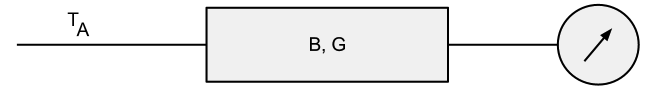
\includegraphics[width=\textwidth]{Images/simple_rad.png}
\isucaption{The ideal radiometer block diagram}
\label{simplerad}
\end{figure}
}

Figure~\ref{simplerad} shows us an ideal radiometer.  That is a radiometer that has an input from the antenna, T$_{A}$, a known bandwidth denoted as B and a known gain denoted as G.  At the end of the block is the detector, which measures the power from the radiometer.

Only a certain selection of the radio spectrum is observed by the radiometer.  This is referred to as the bandwidth of the radiometer and is denoted as B or as $\beta$.  This bandwidth is then centered around a center frequency.  In our scenario, we center around 1.4125 GHz.  There is a reason why 1.4125 GHz is selected and that is from 1.4000 to 1.4250 GHz is protected internationally to be as radio frequency interference free as possible.  This reduces interference from outside sources such as transmitters that can interfere with the operation of the radiometer.  

The power coming from the antenna is amplified so it is easier to determine changes in the brightness temperature.  The overall gain of the radiometer system is referred to as $G$.  Finally, we need to apply Boltzmann's constant, referred to as \textit{k}.  With these values, we can now compute the power the radiometer will see for an ideal radiometer.  This can be shown in equation~\ref{eq:power_rad_eq}

\begin{equation} \label{eq:power_rad_eq}
P=k*\beta*G*(T_{A}) (watts)
\end{equation}

However, since we do not have an ideal radiometer, we have another key component that needs to be addressed.  This is the noise that is added to the system by the radiometer itself, primarily from the amplifiers used to increase the signal.  Most of the additional noise is from the Low Noise Amplifiers (LNA) that are used to increase the signal while attempting to keep the noise added by the LNA to a minimum.  However, noise is also added from virtually every component in the RF front end.  However, by far the largest contribution usually comes from the LNA, which is why the selection of the LNAs is a critical decision.  Figure~\ref{noiserad} shows the additional noise that is injected into the system.

{\begin{figure}[h!tb] 
\centering
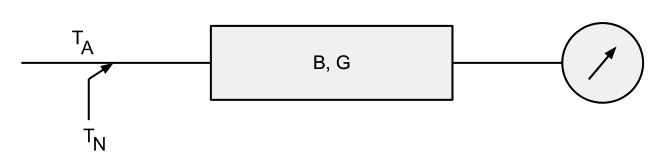
\includegraphics[width=\textwidth]{Images/radiometer_noise_added.png}
\isucaption{A more realistic radiometer model}
\label{noiserad}
\end{figure}
}

As it can be seen, this additional noise is added to the noise coming from the antenna source.  Therefore, T$_{N}$ is added to T$_{A}$ and our final equation for the power measured is shown in equation~\ref{eq:final_power}.  

\begin{equation} \label{eq:final_power}
P=k*\beta*G*(T_{A}+T_{N}) (watts)
\end{equation}

A more typical radiometer can be shown in Figure \ref{trad_radiometer}.  Here we have expanded the blocks used and have replaced the bandwidth block with a bandpass filter which establishes our bandwidth.  Gain is accomplished by using Low Noise Amplifiers (LNAs) that amplify the signal while minimizing the amount of noise they contribute to the system.  Power detection is accomplished typically with a square-law detector and this output is often run through an integrator to smooth the output[\cite{Leinweber}].  Finally we have the output which is a voltage represented as V$_{out}$.  This results in equation~\ref{eq:vout_1}.

\begin{equation} \label{eq:vout_1}
V_{OUT}=c*(T_A+T_N)*G
\end{equation}

Here V$_{OUT}$ is shown by the addition of both the noise from the system T$_N$ and the noise from the antenna, T$_A$ and multiplied by the gain in the system, G[\cite{skou}].  A constant factor $c$ is useful for when we are looking at a radiometer like a Dicke radiometer in which the value of $c$ is $\frac{1}{2}$.  In most applications outside of a Dicke radiometer, $c$ is 1 and can be ignored.  

The voltage output from this radiometer is then either measured or may also be sampled by an analog to digital converter.  This voltage then represents the total power measured by the radiometer, however this measurement is not calibrated.

{\begin{figure}[h!tb] 
\centering
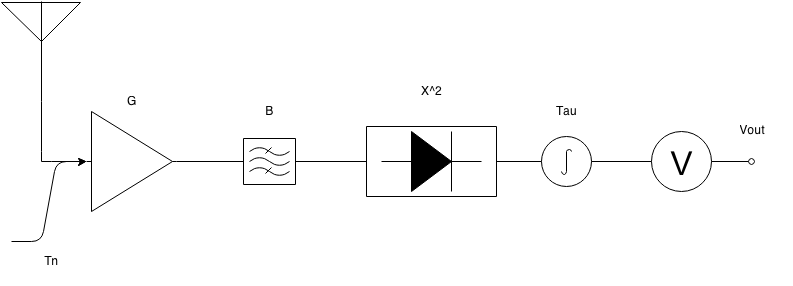
\includegraphics[width=\textwidth]{Images/Radiometer.png}
\isucaption{A total power radiometer block diagram}
\label{trad_radiometer}
\end{figure}
}

Most radiometers are more complicated than the one shown in Figure~\ref{noiserad}.  Additional signal conditioning is often needed which filters and may also amplify or attenuate the signal as required for proper performance through the RF chain.  Once the total power is detected a method to measure and store this reading must also be done.  Finally, additional hardware may be required to stabilize the radiometer which will be discussed in more detail in this thesis.

\subsection{Integration and filtering}

Filtering with a traditional radiometer is usually accomplished by using mechanical filters.  Often these are bandpass filters that limit the bandwidth that the radiometer sees.  Other filters, such as a low pass filter are also used, but usually to smooth out the output from the square law detector.  Another item used to help smooth out the signal from the square law detector is an integrator.

A RC filter is analogous to an integrator where the R and C values determine our time constant and our integration time for the filter[\cite{Aitken}].  We know a RC filter is analogous to an integrator by looking at equation \ref{eq:rc_int}.

\begin{equation}\label{eq:rc_int}
\frac{1}{RC}\int{V_idt}
\end{equation}

To begin with, we look at what an analog RC filter looks like. 

{\begin{figure}[h!tb] 
\centering
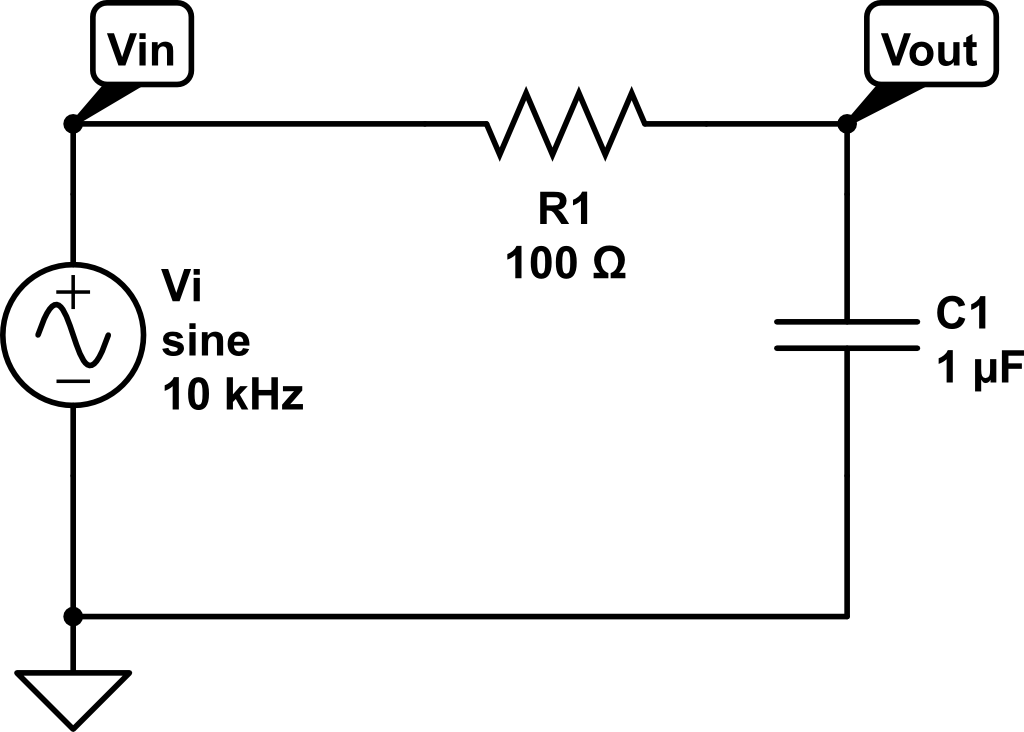
\includegraphics[width=10cm]{Images/rc-circuit.png}
\isucaption{A simple RC circuit}
\label{rc_circuit}
\end{figure}
}

This circuit can be represented by equation \ref{eq:rc_circuit_eq}.

\begin{equation}\label{eq:rc_circuit_eq}
\frac{V_{in}-V_{out}}{R}=C\frac{dV_{out}}{dt}
\end{equation}

\subsection{Radiometer Performance Metrics}
There are two criteria that determines how well a radiometer performs.  The first criteria is with the sensitivity of the radiometer.  This tells us how well the radiometer can differentiate between the information we want and the noise we do not want.  The second criteria is stability.  A radiometer needs to be calibrated to give us useful information.  Stability refers to how much change or drift a radiometer is experiencing which in turn can affect the accuracy of our data.  

\subsubsection{Sensitivity}

Sensitivity of the radiometer relates to the amount of power that the radio selects from the antenna.  This selection is then dependent on the bandwidth that the radiometer is able to listen to.  The radiometer however detects not only the signal of interest but also receives a noise signal as well.  This noise is added to the signal and can not be separated from the signal.  Because this noise is added to the signal, we must be able to determine a change in the signal while the noise signal is also present.  

Power from the radiometer can be expressed in equation \ref{eq:final_power} from chapter 2, where we take into consideration bandwidth, gain and the input from the antenna plus the noise added from the antenna.  

Sensitivity relates to being able to distinguish one signal from the other.  In other words, we must be able to distinguish, or detect, our wanted signal from noise that is present in the signal.  To demonstrate this, consider a system that has a system noise temperature of 700K and an antenna temperature of 300K.  This gives us a total noise temperature of 1000K.  Therefore, if we wish to detect a change of 1K, we need to be able to detect between 1000K and 1001K.

Since our signal is really random fluctuations about a mean power input to our system, we can reduce the fluctuations by averaging or integrating the signal.  This results in equation \ref{eq:rad_sensitivity} which is derived in chapter 2.

\begin{equation} \label{eq:rad_sensitivity}
\Delta T=\frac{T_{A}+T_{N}}{\sqrt{\beta * \tau}}
\end{equation}


This equation gives us the radiometer sensitivity based on the input, which is both the noise and input signal with consideration to the bandwidth and integration time, or averaging, that is done to the signal.  


The issue with all radiometers is that it must detect small signal changes in a noisy environment.  To understand this, let us look at the example of T$_{A}$ has a value of 200 K and T$_{N}$ has a value of 800 K.  Since T$_{N}$ is added to our antenna signal, we have a total noise temperature of 1,000 K.  This means that if we want to detect a change as small as 1 K, we must be able to measure the difference between 1,000 K and 1,001 K[\cite{skou}].

The ability of a radiometer to detect these small changes is the radiometer's sensitivity, or the standard deviation of the output signal from the radiometer.  This sensitivity is also referred to as the Noise Equivalent Delta ($\Delta$) Temperature or NE$\Delta$T and is shown in equation \ref{NEAT_EQ}. 

\begin{equation} \label{NEAT_EQ}
NE\Delta T=\frac{T_{A}+T_{N}}{\sqrt{\beta * \tau}} 
\end{equation}

The sensitivity of the radiometer is based on both the bandwidth, $\beta$, of the incoming signal and the integration time, $\tau$.  As it can be seen in the equation, we want to have as much bandwidth as possible.  In a traditional radiometer, this bandwidth is often fixed and is dependent on the band-pass filters used in the radiometer.  We can however control $\tau$ and a longer integration time will help improve the sensitivity of the radiometer to a certain degree.[\cite{ulaby}]

\subsubsection{Stability}
Stability and accuracy are additional problems that need to be considered when looking at the radiometer system.  To begin we can once again look at the power received equation that we discussed in Chapter 2 and is equation \ref{eq:final_power}.

As we look at this equation, we can see that if $k$, $\beta$, $G$, and $T_{N}$ are constant, then stability can be assured.  The Boltzman constant $k$ is a known constant and we can also assume that our bandwidth, $\beta$, will also remain constant.  Gain and the noise temperature however will vary.  

Gain is usually our largest factor that can change on a radiometer and even with a software defined radio this is still a large source of variation.  This is due to the analog nature of the amplifiers that affect a large portion of the gain in our system.  Various things can affect our gain but the two largest factors is the physical temperature of the amplifier and the voltage that feeds the amplifier.  Voltage can be controlled to a degree.  High accuracy voltage regulators can help control fluctuations in voltages that can in turn affect the gain.  A factor however that is harder to control is temperature.  It can be seen in equation \ref{eq:rad_stability} that temperature change due to gain fluctuations us directly related to the changes in gain and the overall gain of the system. It is because of this that the current ISU radiometer has gone to great strides to control the temperature of the amplifiers to maintain a constant temperature.

\begin{equation} \label{eq:rad_stability}
\Delta T_G=T_{sys} \left(\frac{\Delta G}{G}\right)
\end{equation}

To verify stability of the radiometer, we look to see how much change the radiometer records over a relatively long period of time.  To test this a matched load was submerged in a liquid nitrogen bath for an extended period of time, in this case for fifteen minutes.  The readings were then looked at to study the trend of the data.  The data is graphed in figure \ref{Stability}.

\begin{figure}[h!tb] \centering
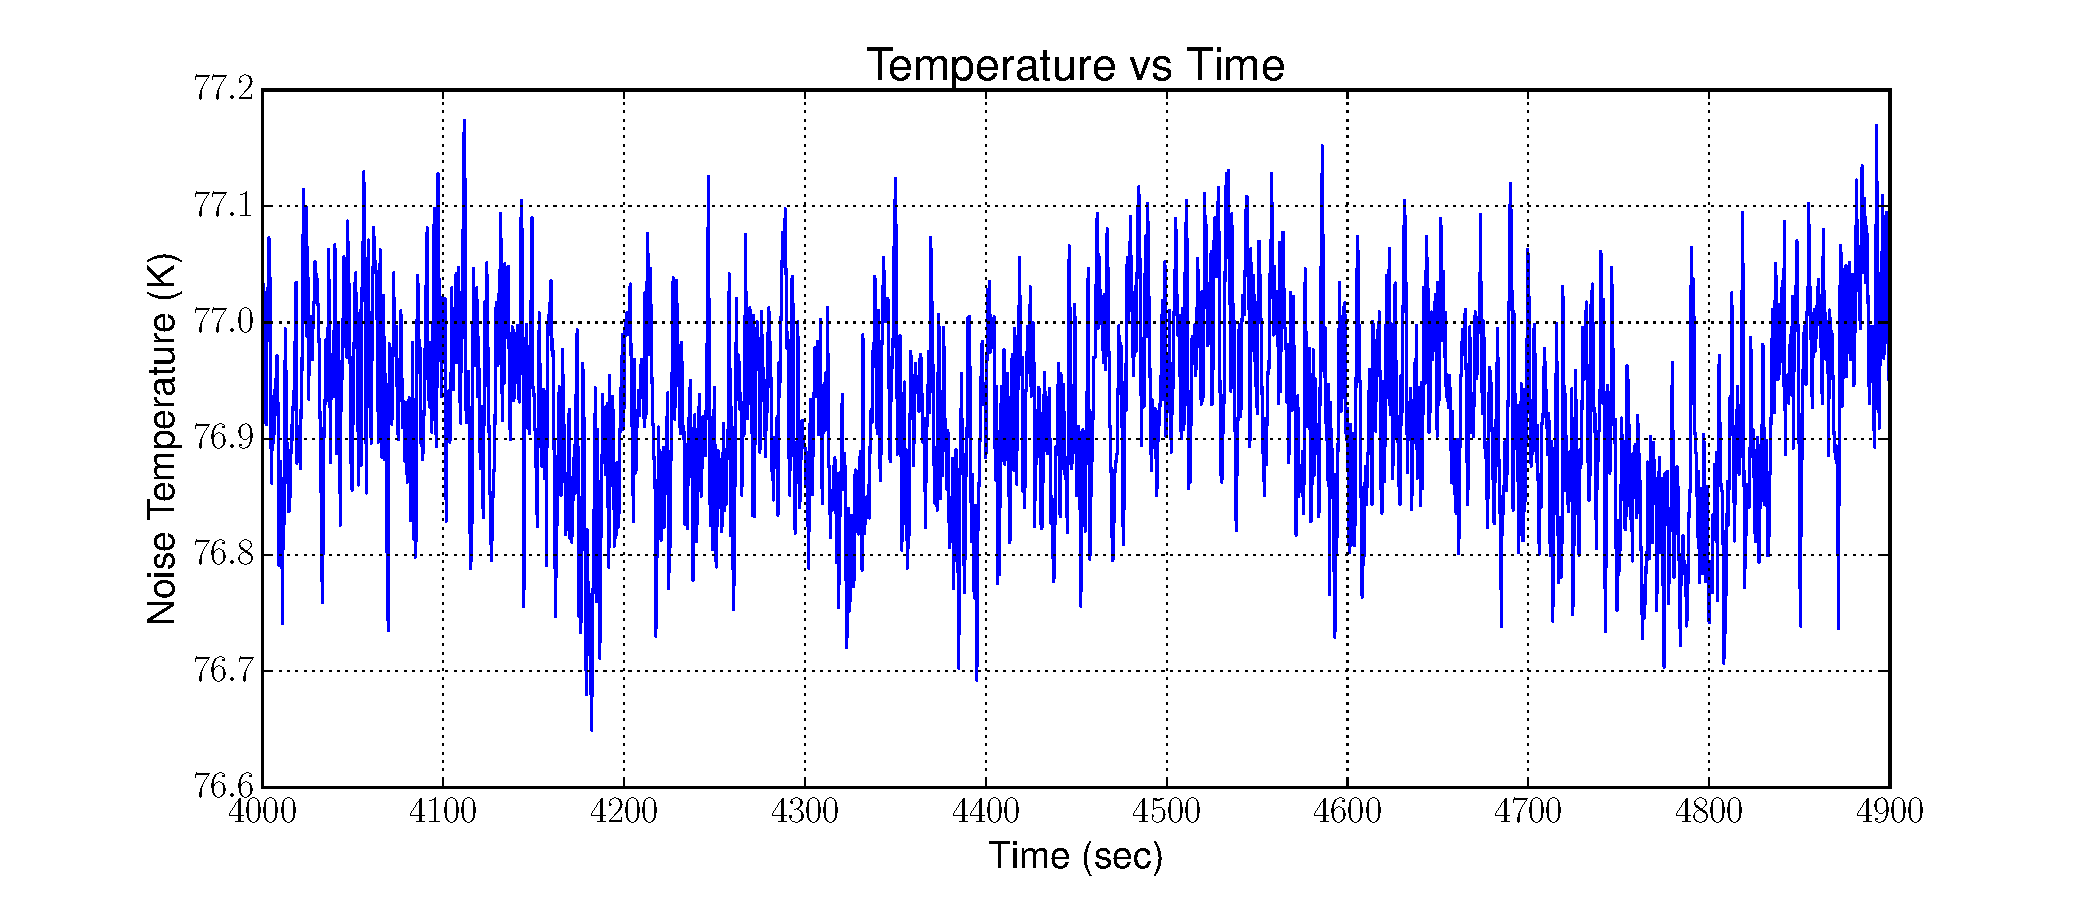
\includegraphics[width=\textwidth]{Experiments/Exp2/sdr_calibrated_zoom.pdf}
\isucaption{Graph of the calibrated total power over a period of fifteen minutes.}
\label{Stability}
\end{figure}

\begin{figure}[h!tb] \centering
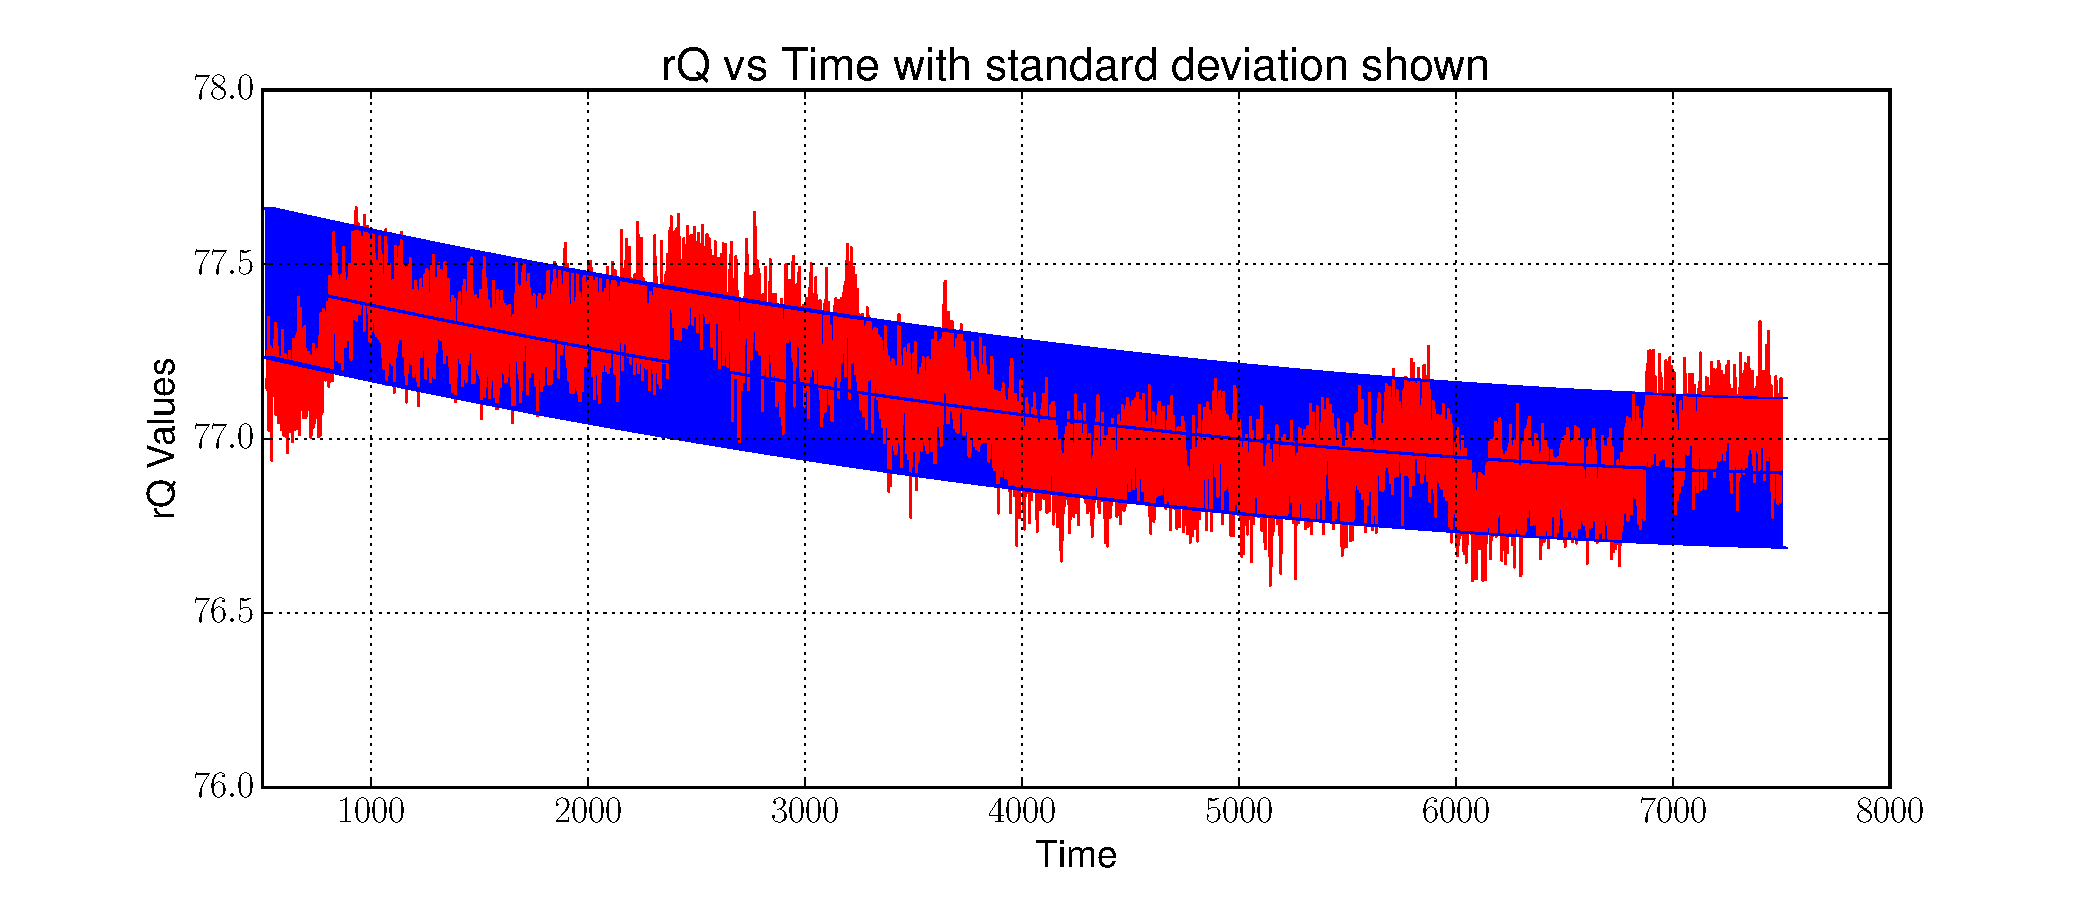
\includegraphics[width=\textwidth]{Experiments/Exp2/calib_vstime_stddev.pdf}
\isucaption{Graph of the calibrated total power with the standard deviation plotted.}
\label{Stability_calib}
\end{figure}

As it can be seen in figure \ref{Stability}, the amount of change over a period of one hour is quite small.  The standard deviation for this sample is 0.09 kelvin.  The $NE\Delta T$ calculated using 10 MHz for the bandwidth, an integration time of 2 seconds and with our sample at 77 Kelvin is calculated to be 0.10 Kelvin with a system temperature of 350 Kelvin.  Therefore, our system is behaving as we expect it to for this stability test.

Figure \ref{Stability_calib} shows a graph of the total readings but with the standard deviation now plotted.  This shows that the system is stable and is operating as expected within our expected $NE\Delta T$.

\subsection{Implementation of traditional radiometer}
 
\section{Software Defined Radios Basics} 
Software Defined Radios (SDRs) are used for a variety of applications but their primary application has been in the area of communications.  They appeal to applications where being able to change a modulation scheme or filter on the fly is desirable.  In these areas, SDRs often outperform a traditional hardware only radio with their ability to rapidly change their operations by simply changing their software.  Early SDRs were expensive due to the high costs in the analog to digital converters (ADCs) needed and in the high speed Field Programmable Gate Arrays (FPGA) used.  In recent years however, the cost of SDRs have decreased due to the cost of these key components decreasing in cost as well.  Even though the cost has gone down the performance of SDRs have increased and this has lead to new developments in applications for using SDRs in new and different ways.

The basic concept behind a SDR is that it will digitize the RF signal as soon as possible.  Once digitized, it is now evaluated by a computer, FPGA, or a dedicated System on Chip (SoC).  A canonical software defined radio architecture is one that consists of a power supply, antenna, multi-band RF converter, and a single chip that contains the needed processing and memory to carry out the radio functions in software [\cite{Mitola1995}]. This allows us to extract certain hardware functions, such as filtering, into the digital domain which can then be manipulated by software.  Since software is now manipulating the signal, we can rapidly change what functions we execute on the signal by changing the software.  This gives SDRs a high amount of flexibility as components that are normally done in hardware can now be done in software and can be changed by simply uploading new software or firmware to the system.  This also gives us a benefit in cost as certain components are no longer needed and changes done in software do not require additional hardware to be added or to be swapped out.

\subsection{Software Defined Radio Normal Operation}

\section{Software Defined Radio Development Platform}
The work of this thesis is to use an off the shelf software defined radio (SDR) to perform the same operation or better of a traditional analog radiometer.  Using a SDR radio also means that we are able to be more flexible in how the radiometer performs, is capable of frequency agility and adapting to changing conditions such as interference.  Using a software defined radio also allows for implantation of different radiometer types such as a polarimetric radiometer, a correlation radiometer and also a polarimetric radiometer that uses Stokes parameters [\cite{Wang}].  Normally, these require changes to hardware, but all of these types of radiometers can be implemented in software increasing the flexibility of the system.  
\subsection{Hardware Platform}
The key component for a software defined radio radiometer is the software defined radio or SDR that will do most of the work as a radiometer through software.  The equipment selected for researching into this topic was the Ettus Research Group N200 SDR.  The SDR selected utilizes daughter boards as the RF front end to the SDR and up to two daughter boards may be installed into a N200.  This is an important consideration as one of the requirements is to be able to look at both the V-Pol and the H-Pol signal coming from the antenna.  By having a dual receiver SDR it is possible to correlate the signal and other signal analysis can also be done.  Another important reason the N200 is selected was due to its ability to handle up to 50 MHz of bandwidth to the computer and up to 25 MHz of RF bandwidth per daughter-board plugged in to the SDR.  This means that it is possible to have two receive cards that can stream up to 25 MHz bandwidth each.  

The N200 utilizes a flexible architecture for a variety of RF interface systems based on the frequency range desired and if receive and/or transmission is needed.  These daughter boards directly receive the RF signal and then outputs the analog I and Q signals that are then sampled by the N200 A/D converter for reception or receives the I and Q values from the N200 D/A converter for transmission. 

{\begin{figure}[h!tb] 
\centering
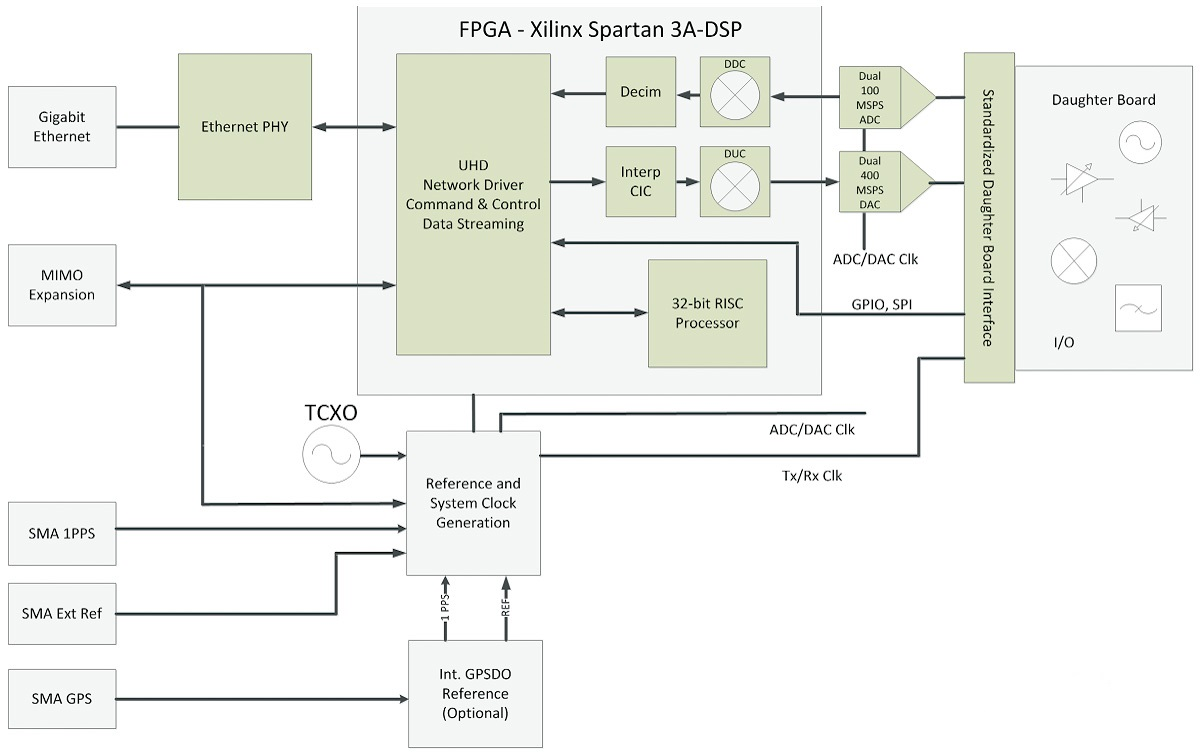
\includegraphics[width=14cm]{Images/n200_block_edited}
\isucaption{A block diagram of the Ettus N200 SDR}
\label{N200_block}
\end{figure}
}

The daughter board selected is the DBSRX2 card as this card is receive only and operates between 800 MHz and 2.4 GHz.  The DBSRX2 also has built in amplification that is adjustable through software.

The hardware that was selected for this research was the Ettus Research N200 Software Defined radio.  The N200 is a research designed hardware that gives us the standard building blocks for a typical software defined radio which includes an A/D converter and on-board FPGA.  The N200 however, also gives a flexible front end by selecting daughter boards that fit our application.  In addition, the N200 supports up to two daughter boards to be installed. 

{\begin{figure}[h!tb] 
\centering
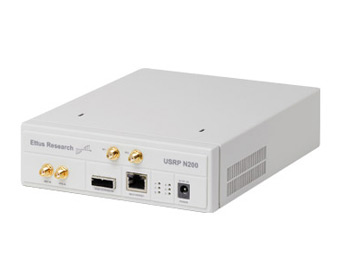
\includegraphics{Images/n200}
\isucaption{The USRP N200 from Ettus Research (Image from Ettus Research Website - www.ettus.com)}
\label{N200}
\end{figure}
}

The N200 has the following features that made it well suited for our specific application.

\begin{itemize}
\item Dual 14-bit ADC
\item Dual 16-bit DAC
\item 50 MS/s Gigabit Ethernet streaming
\item Modular daughter-board system for RF front end
\end{itemize}

These specifications had a large impact on the selection of the N200 for this application.  Specifically the 14-bit ADC, the 50 MS/s and the modular daughter-board system were the largest factors in the decision to use the N200 SDR.  Further explanation on these specifications are explained in the following sections.

\subsubsection{14-bit ADC}
The analog to digital converters (ADC) allow us to take the analog I and Q values from the daughter boards and digitize this information.  Once digitized, we can now work with the signal both on the on-board FPGA board or stream it to the computer so that our software can manipulate the signal.  In radiometry, we are primarily looking at the overall power of the signal and this does not require us to accurately recreate the signal.  However, as will discuss later there are times were we do want frequency information and having an accurate frequency representation of the signal will then be an important factor.

\subsubsection{50 MS/s Bandwidth}
For this application, the N200 is required to receive a signal at 1.4 GHz and is at least 20 MHz wide.  Bandwidth plays an important role in remote sensing and to the amount of power that we receive.  It also plays a key role in the sensitivity of the radiometer.  This was discussed in the theory of a traditional radiometer and equation \ref{eq:final_power} shows us the relationship that our bandwidth plays in the overall power received.    

An equally important consideration is the sensitivity or how small of a change the radiometer can detect.  This sensitivity or NEAT function is shown in equation \ref{NEAT_EQ}.  For this reason the amount of bandwidth that the SDR can handle is another specification that had to be considered.  

Another factor however is the amount of bandwidth the existing RF front end of the ISU radiometer is able to provide to us.  The current filters on the ISU Radiometer keep the bandwidth of the signal to 20 MHz.  This meant that a minimum of 20 MS/s bandwidth from the SDR is required.  

The N200 is capable of working with up to 100 MS/s signal and can stream up to 50 MS/s through the Gigabit Ethernet connection.  The N200 also has the ability to have up to 2 daughter boards installed.  If we assume each will have up to a 20 MHz signal, this means up to 40 MS/s of data will be required.  This means that the N200 meets and can exceed the bandwidth requirements that we were looking for.  In addition, the FPGA on the N200 is capable of working with up to 100 MS/s, so there is room handling additional bandwidth by using the on board FPGA to process the signal.

\subsubsection{The DBSRX2 Receiver}

The Ettus Research N200 SDR uses daughter boards which allow for easy replacement of the RF front end to the software defined radio.  Ettus Research makes a number of daughter boards that range from a wide range of frequencies and is available with transmitters, receivers and transceivers.  Because these boards are modular and do not touch the analog to digital converters or the on-board FPGA, little change is required in the software.  The daughter boards however do have the required RF hardware for the signal to be processed.  In this application it was required that the signal was detected at 1.4 GHz with a bandwidth of 20 MHz.  The DBSRX2 receiver met this requirement and was selected to be used with the N200.  In this radiometer application transmission is not needed and is illegal in the 1.4 GHz band, which is reserved for passive radiometer applications.

The DBSRX2 receiver board is capable of receiving signals between 800 MHz and 2.3 GHz.  The board is able to plug into one of expansion slots available on the N200 that we are using.  This board then down-coverts the signal into analog I and Q values that are then fed into the N200 analog to digital converter.

{\begin{figure}[h!tb] 
\centering
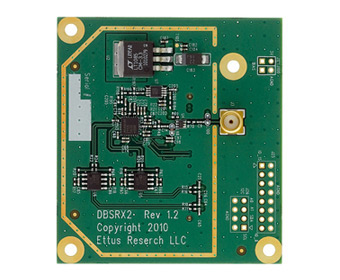
\includegraphics{Images/dbsrx2.jpg}
\isucaption{The DBSRX2 daughter board from Ettus Research (Image from Ettus Research Website - www.ettus.com)}
\label{dbsrx2}
\end{figure}
}

The DBSRX2 has several key components on it that is used to take the analog RF signal and prepare it for digitization by the analog to digital converter.  First the signal is amplified through a Programmable Gain Amplifier (PGA).  This PGA is accessible from the software and can be configured by the software.  Next the signal goes into a direct-conversion integrated circuit that directly converts the RF signal to analog I and Q values.  The integrated circuit, a Maxim MAX2112 device, also includes a Low Noise Amplifier (LNA), mixer and Low Pass Filter (LPF).  This essentially amplifies the signal, mixes into baseband and then applies a low pass filter.  

{\begin{figure}[h!tb] 
\centering
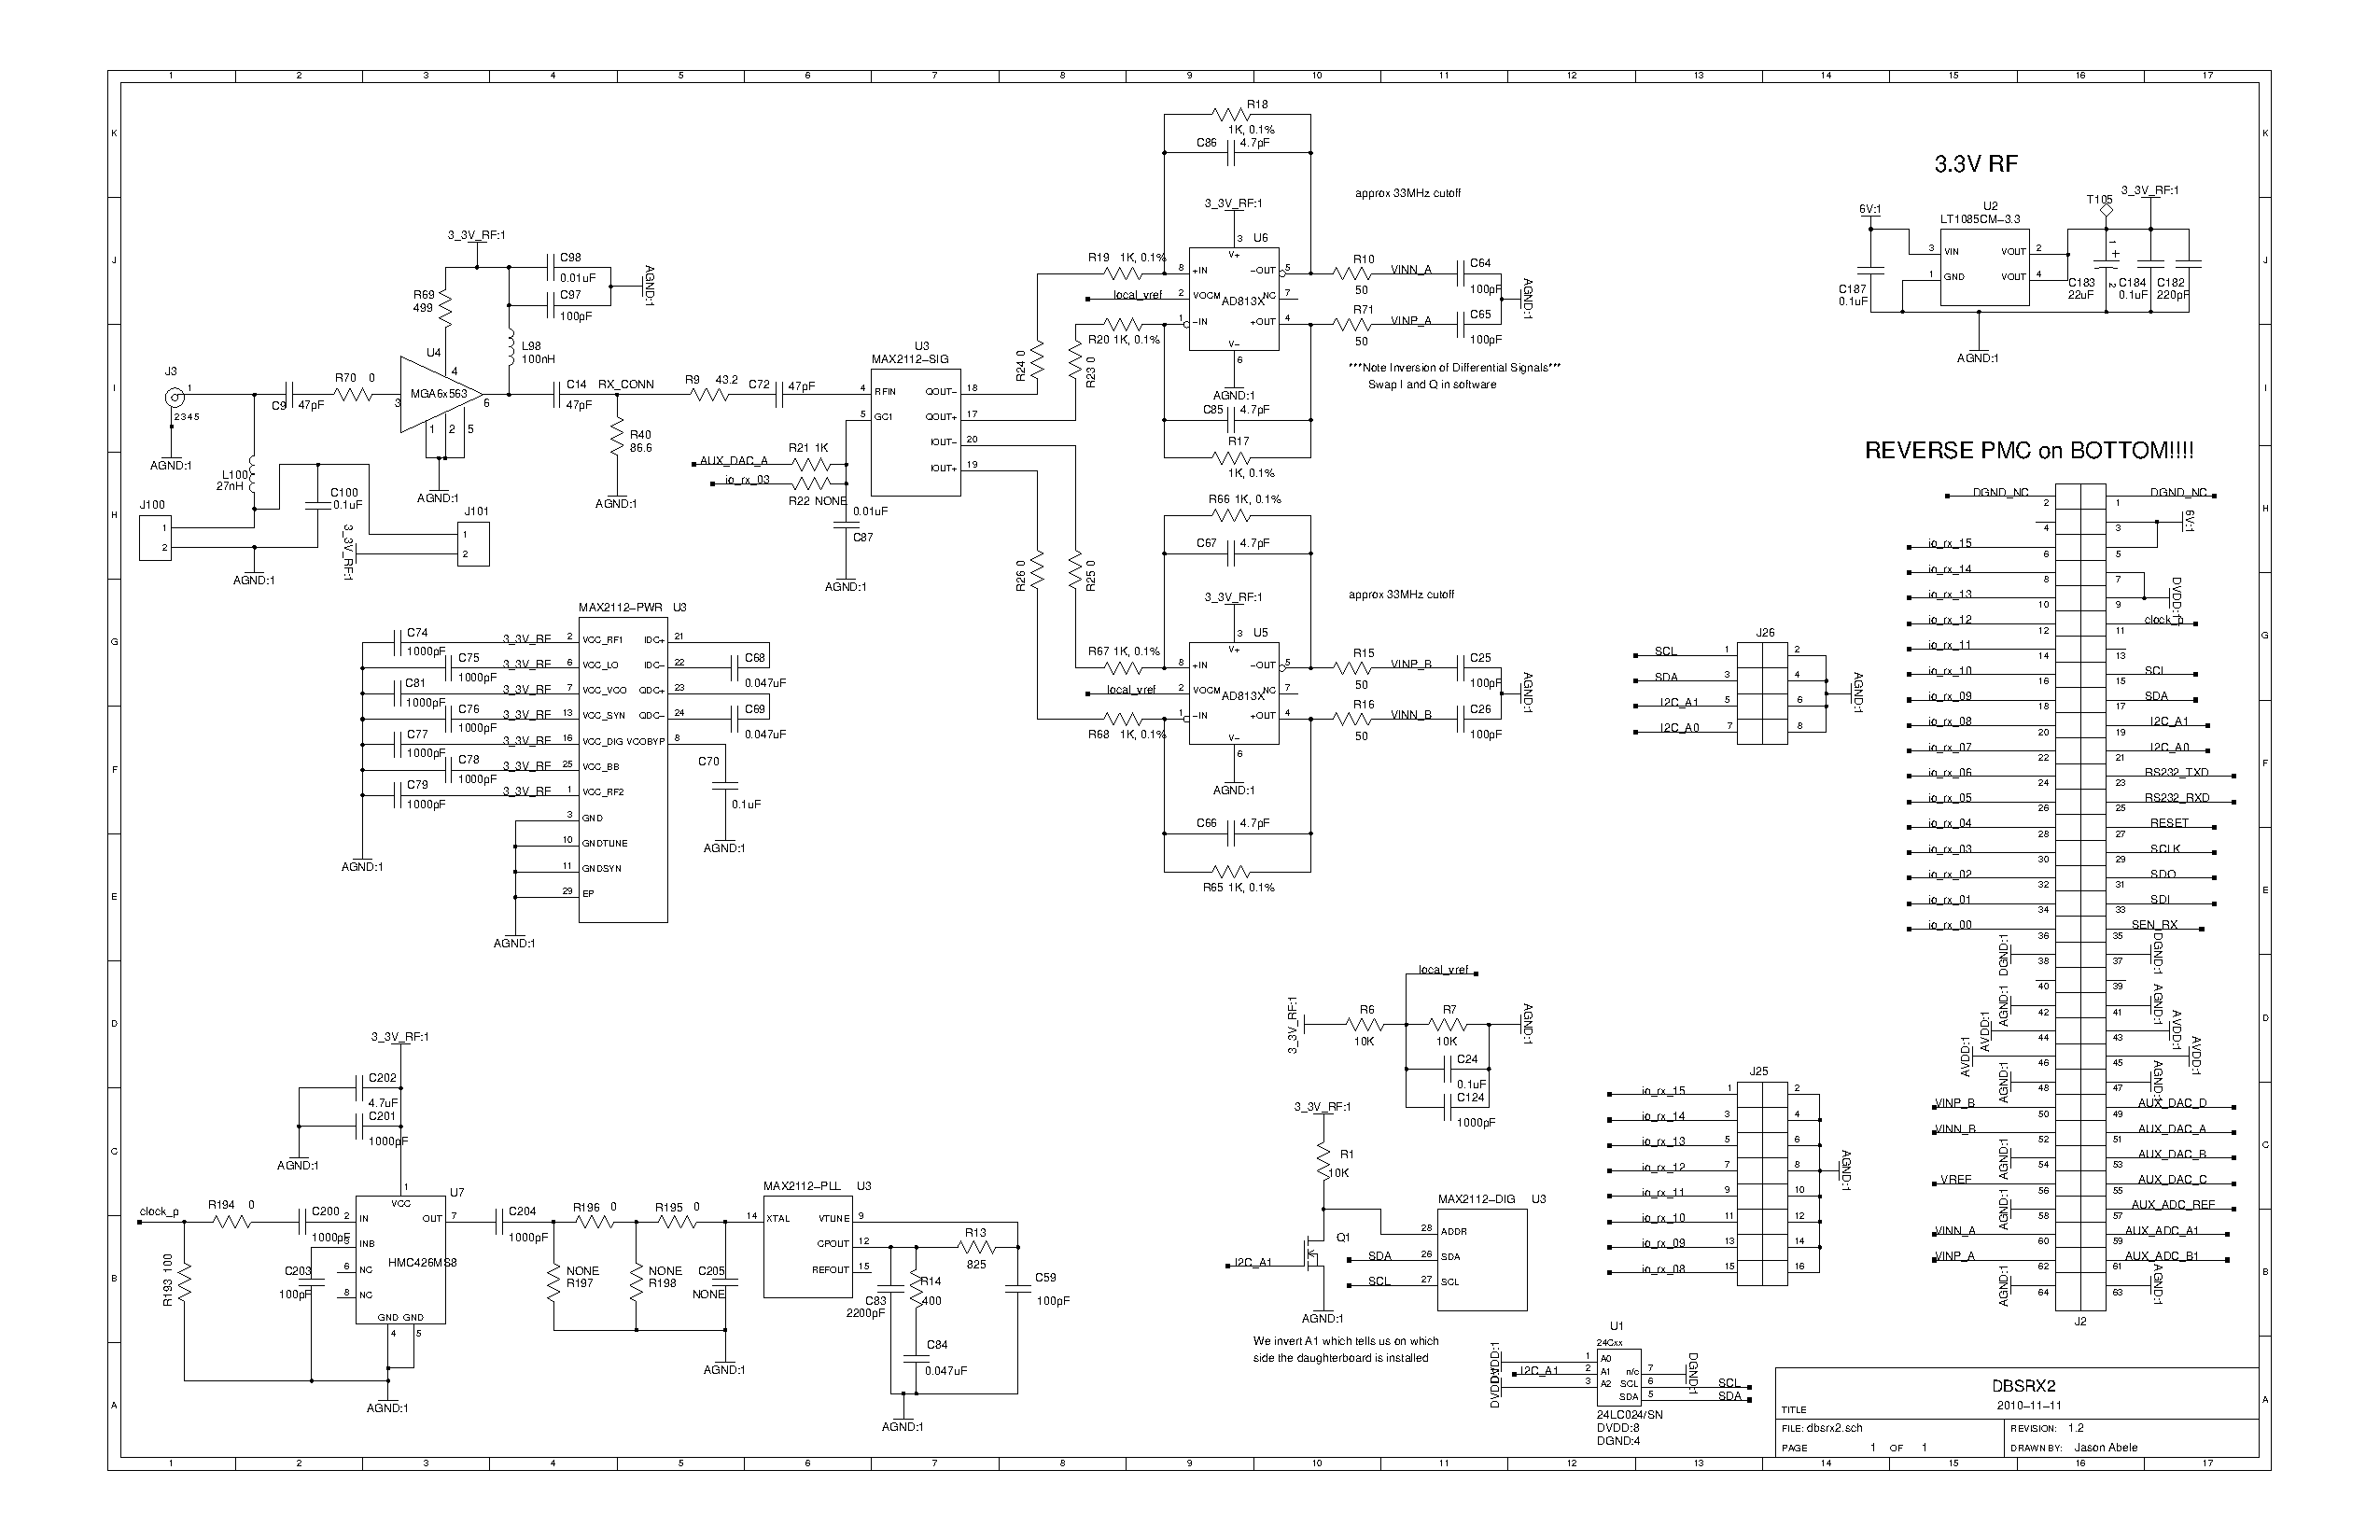
\includegraphics[width=\textwidth]{Images/dbsrx2.pdf}
\isucaption{The DBSRX2 Schematic (Image from Ettus Research Website - www.ettus.com)}
\label{dbsrx2_sch}
\end{figure}
}

These analog I and Q values are then passed to the N200 to be sampled by the analog to digital converter.  The IQ values are differential signals to minimize noise possible interference.

\subsubsection{DBSRX2 Noise Temperature Consideration}

The N200 uses daughter board cards that allow for us to easily swap out different RF front ends.  The DBSRX2 was selected since it is receive only and that it will work in the frequency spectrum that we are interested in which is in the 1.4 GHz range.  Since we are using the DBSRX2 after the LNAs that are already in use, the noise temperature added by the DBSRX2 will be small.  The DBSRX2 adds approximately 5 dB to the noise factor of the system.  Again though, since this is at the end of the RF chain, the total contribution of the DBSRX2 to the overall system noise temperature is small, and has been calculated to be 1.05 dB to the overall noise factor of the system.

While the DBSRX2 does have additional gain, this gain is not as critical since we have the additional gain from the ISU radiometer front end.  While the gain the DBSRX2 is significant, the noise figure on the DBSRX2 by itself is high.  Therefore, the DBSRX2 is not a good candidate if the N200 is used solely by itself.  Ideally, there is at least one if not multiple LNAs that have much better noise figure numbers than what the DBSRX2 and is placed in front of the DBSRX2 daughter-board. 

\subsection{Software Platform} 

Software of course plays a critical role in a software defined radio and also in our software defined radio radiometer.  There are two pieces of software that are in play with the software defined radio we are using.  The first is the firmware that is used in the FPGA of the N200.  This firmware provides low level processing of the signal so it can be sent to the software located on the computer.  It also provides a link for controlling key aspects of the software defined radio such as additional gain, bandwidth and the center frequency.

The second is the software that is running on the host computer.  It is this software that provides the calculations on the I/Q data to give us the information we need and also creates a GUI for the user to interface with the radio.  For this software, we will be using GNURadio, an open source software program that is used in software defined radios including the N200 SDR that we have.  

For the computer, GNURadio will be used to do all signal processing that is needed.  GNURadio is an open source software define radio framework that runs on multiple OSes and offers a rich set of features.  In addition, GNURadio is well supported by the Ettus Research group and is the preferred software for interfacing with their hardware.  An easy to use interface was another driving requirement for our implementation of a radiometer in a SDR.  GNURadio helps us with this through the use of the GNU Radio Companion or GRC.  This was important as it was anticipated that operators of the radiometer have a limited knowledge about programming.  GNURadio uses a simple to use graphical system that is similar to things such as LabView, offering a drag and drop system for adding radio components such as filters.  Like LabView, you can also simply wire up the boxes and complete the circuit path for the RF signal as it gets processed.

GNURadio fills in the software side of the software defined radio.  Although there is firmware that runs on the FPGA in the N200, this firmware is designed to communicate with a host PC.  It is this software that does most of the work by doing the calculations that apply to the signal.  The FPGA simply sends the raw IQ data to the host PC, which then performs the necessary math functions.  Again, the reason why software defined radios are desirable is the ability to change the behavior of the radio quickly.  In our scenario we can change functionality by simply loading a new software program in the host PC.  

This functionality is ideal for communication type of radios where different modulation schemes and encoding and decoding methods can easily be changed out.  However, in a radiometer we are not interested in this aspect of the SDR.  However, one functionality is available that can be valuable for a radiometer, and that is with filtering.  Although we often use frequencies that should be free from interference, this is not always what happens in the real world.  Interference can and often does still occur, even in these protected frequencies.  With the SDR, we are able to quickly adapt to changing conditions by moving the frequency, changing our bandwidth and even filter out an offending signal.  

GNURadio was selected as it is an open source software platform.  GNURadio is licensed under the GPL license and has a strong community that continually updates the software.  It is also well supported by third parties such as Ettus Research Group, National Instruments and other SDR developers.  In addition, GNURadio has a strong set of tools that can be used to develop programs that run under GNURadio.  Tools such as the GNURadio Companion (GRC) allows for an easy to use GUI to develop code for GNURadio.  GNURadio is also written in Python, which allows for easy modification and access to additional tools that can be used with GNURadio.  

{\begin{figure}[h!tb] 
\centering
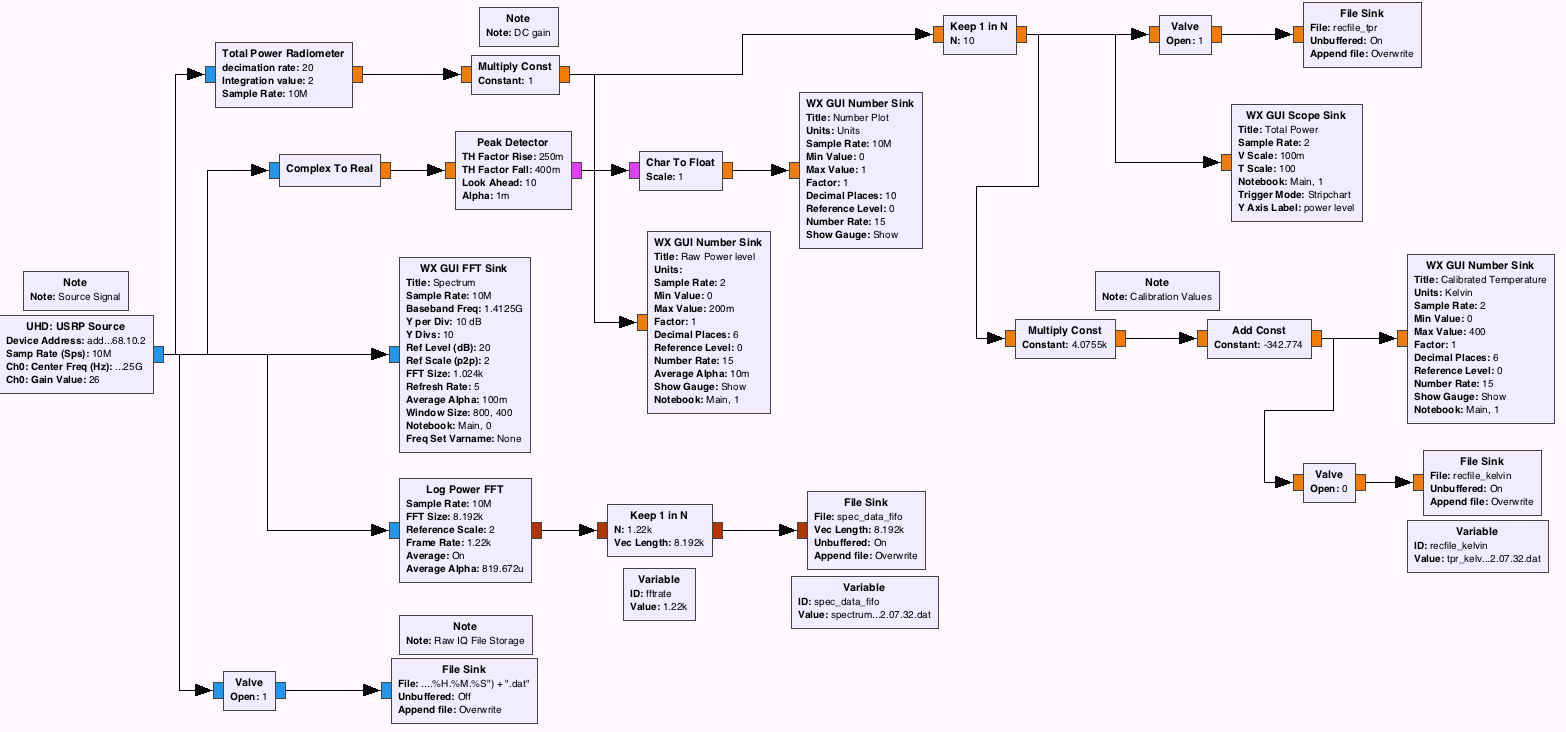
\includegraphics[width=17cm]{Images/N200_radiometer_grc.png}
\isucaption{Screenshot of the GNURadio Companion editor and the N200 Radiometer block diagram used in the author's experiments}
\label{N200_GRC}
\end{figure}
}

GNUradio Companion works by having the common functions as blocks that can picked and placed on the screen.  Once placed, the blocks can be wired up, much like LabView, and the flow of data can be controlled in this fashion.  While GNURadio Companion provides most of the essential blocks used in most applications additional blocks can by added if needed.  This is because GNURadio is built using Python and the blocks in GNUradio Companion are simply blocks of Python code.  To compile a GNURadio Companion flow diagram, you simply run the sheet, which then generates the Python code that is then executed.  GNURadio actually uses a combination of Python and C++, where Python handles most of the interface and the C++ is usually most of the drivers and low level interface to the hardware.  This allows for an easy to use system but still meets the demanding performance needed for handling large amounts of data.  

GNURadio Companion also includes blocks that allow it to create a GUI type of interface.  The typical method it uses for this is using wxGUI although GNURadio Companion does also include blocks that can use QT for generating widgets as well.  However, the wxGUI tends to work better and has better support in GNURadio than QT.  

Through these blocks we are able to only manipulate the data we need to perform a total power radiometer in software but to also create a user interface that allows us to control the radiometer as well.  We are also able to display the information in real time so the user can see changes in power and even monitor spectral information during the operation of the radiometer. 

\subsection{Control of the SDR Hardware through GNURadio}
The N200 sends all data across the 1 Gbps connection to be read in by a host computer running GNURadio.  This data is the raw I/Q values that is read by the on board A/D and processed by the on board FPGA.  An example of a very simple GNURadio software implementation would simply take this data and store the data to a hard drive in a file.  This can be very handy if we want to simply record the data and then process it later.  However, depending on the sample rate, it can consume a large amount of storage.  A short recording can easily consume 1-2 GB with a sample rate of 10 Msps.  It also does not give us any immediate feedback on the radiometer and it does not give us controls of the radiometer such as frequency, integration time or other key variables.  Fortunately GNURadio has tools that allows us to build up a very rich application that is able to give us the data we need and control the software defined radio as well.

The GNURadio Companion allows us to create python code that is used to not only receive the data from the SDR but also perform signal processing on the incoming information.  Additional controls are added that allow for tuning of the signal processing parameters and control of the radio functions.  This allows us to build up an application that can be run on any computer that is capable of running GNURadio.  

{\begin{figure}[h!tb] 
\centering
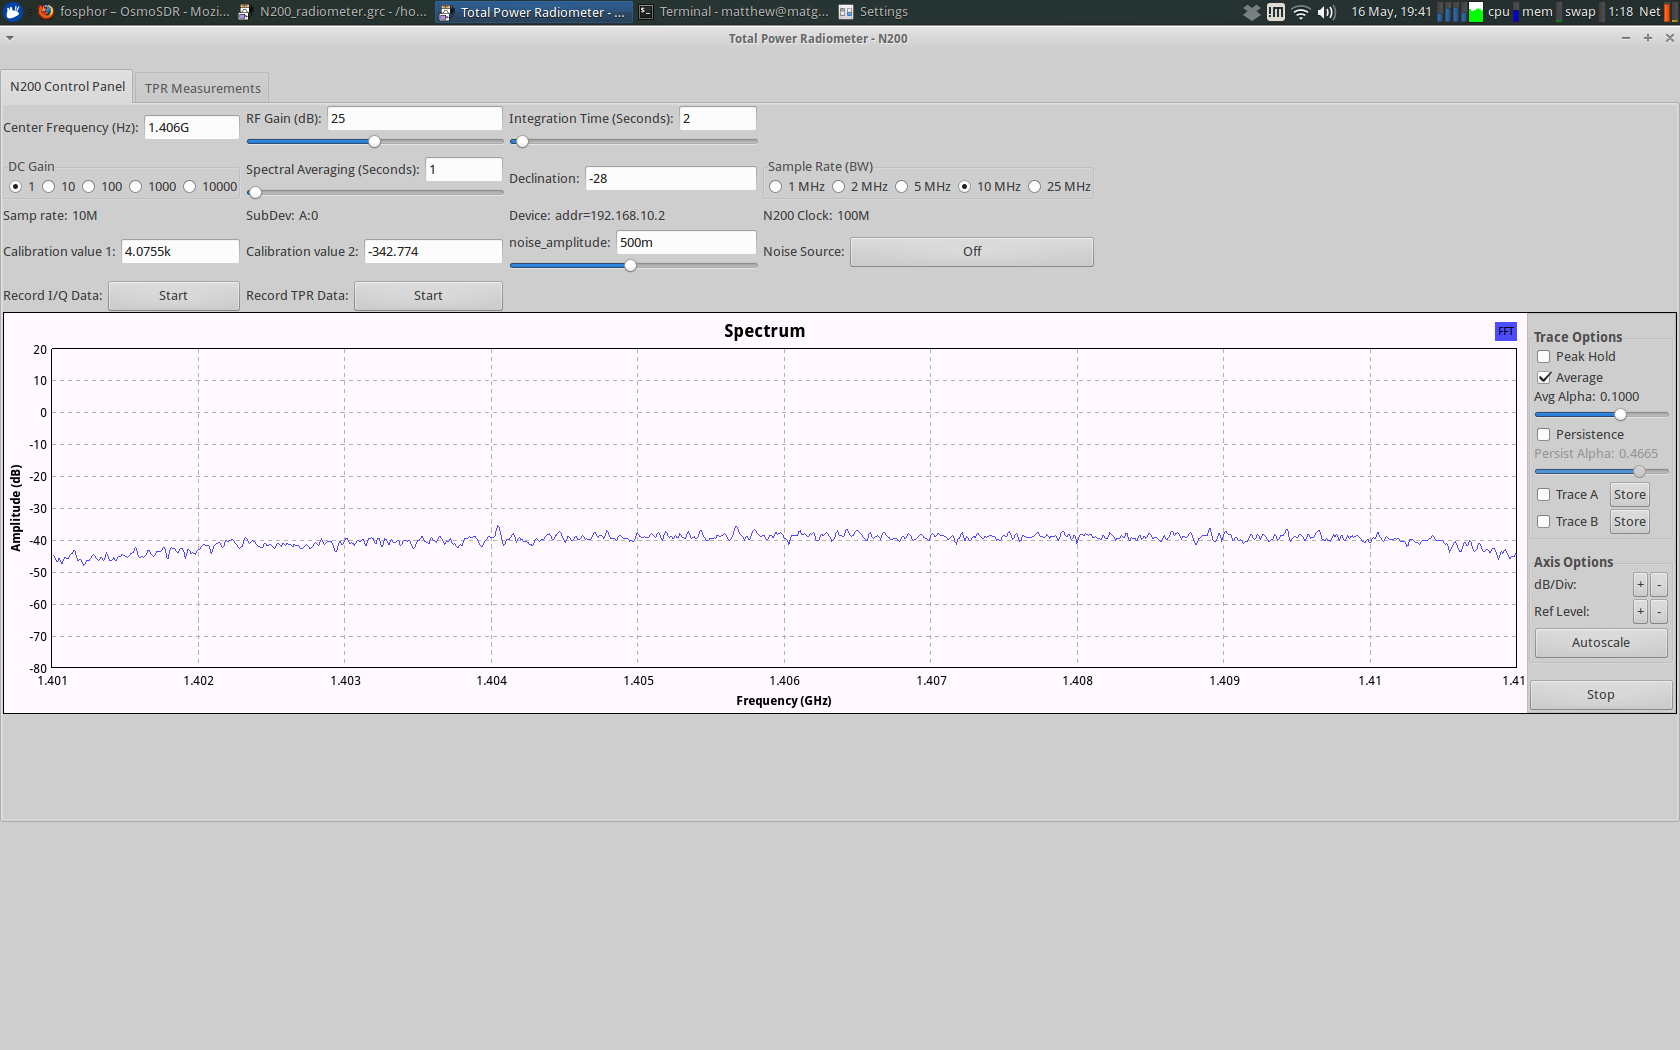
\includegraphics[width=17cm]{Images/radiometer_gui.png}
\isucaption{A screenshot of the interface made for communication with and controlling the software defined radio}
\label{radiometer_gui}
\end{figure}
}

Through this interface we are able to control several key aspects of not only the radio hardware within the SDR but also with the behavior of the radiometer as well.  Hardware control of the SDR hardware allows us to change frequency and also adjust gain values within the N200.  Bandwidth is another parameter that can be altered from here as well.  Bandwidth affects the bandwidth for the RF signal, but also has an impact on the radiometer sensitivity as well.  Additional controls allows for alterations to the radiometer and includes being able to adjust the integration time of the radiometer.  

\subsection{Impact of the Controls Related to Radiometry}

The controls that have been added for controlling the radiometer can have a large impact on the performance of the radiometer.  There is a reason why these controls were added to the GUI for the radiometer and that is they play key roles in how the radiometer performs.  

For any radiometer noise temperature is a large consideration and is critical to the design of the radiometer.  One method to determine how well a radiometer is to look at the sensitivity of the radiometer.  We can do this by looking at the smallest change in temperature the radiometer can see.  We will call this the Noise Equivalent $\Delta T$ or $NE\Delta T$ of the radiometer.  The equation for this is shown below.

\begin{equation}
NE\Delta T=\frac{T_{A}+T_{sys}}{\sqrt{\beta * \tau}}
\end{equation}

$\beta$ can be changed by changing the sample rate of the SDR.  The sample rate effectively controls the bandwidth in which the SDR is operating at.  This also gives us a band-pass filter as well, since the SDR will not respond to frequencies outside of this bandwidth.  

$\tau$ is the integration time for the radiometer.  This parameter is set by the user through the GUI and allows us to change the integration time in seconds.

\section{GNURadio Data Handling}
Once we have the data that has been processed by the software defined radio we will want to display this information and be able to store the data so we can analyze it later if needed.  Data display can be handled GNURadio where we can plot the total power over time.  This allows the user to be able to visualize the total power and be able to determine if the total power has increased or decreased over the time window shown.  

Although not usually needed for a total power radiometer we also have the ability to look at the signal in terms of a frequency versus amplitude.  This allows looking for any unusual signals that may be interfering with the system or causing erroneous data with our radiometer.  

Finally, we will want to store the data so we can do additional analyses on it at a later time.  The GNURadio program allows us to store the data in two formats.  The first format is storing the raw I/Q data from the radiometer.  This format allows us to playback the data through GNURadio at a later time.  This can be useful for if we wish to change parameters in GNURadio such as bandwidth or integration time.  It is also a good diagnostic tool as we can check that the signal coming in is clean or if we need to apply additional filters to remove an unwanted signal. This file may be quite large, consuming several gigabytes of data for a 20 MHz wide signal in a matter of minutes of record time.

The second format is the total power that has been calculated by the radiometer.  This file is much smaller since much of the signal information has now been reduced to simple power versus time information.  This allows for easy manipulation through any math program such as Matlab for analysis.  

\subsection{GNURadio Data Display}
The information from the software defined radio can be displayed through GNURadio to show a number of things.  Since we have both frequency and magnitude information we can display this information.  We are able to also display the information that shows the total power that is being seen by the radiometer as well.

{\begin{figure}[h!tb] 
\centering
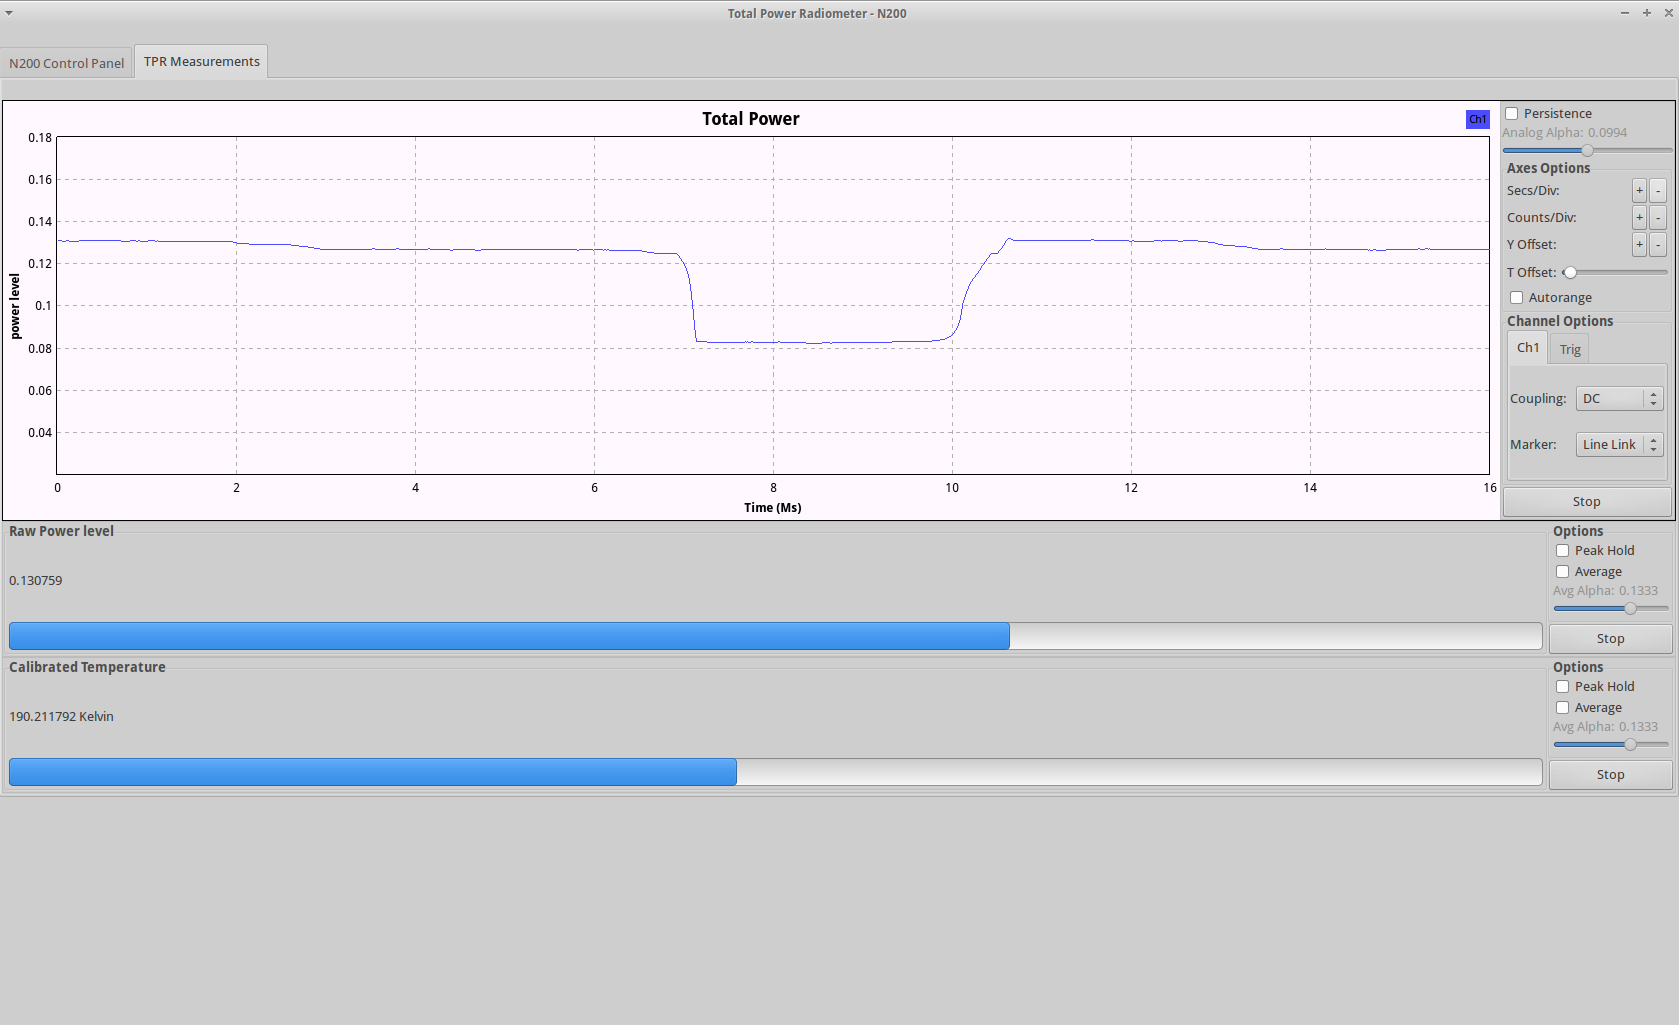
\includegraphics[width=17cm]{Images/Lab1_TPR_at_end_exp.png}
\isucaption{A screenshot showing the ticker tape display for the total power readings.  In addition, raw and calibrated noise temperature is shown below.}
\label{radiometer_tpr_display}
\end{figure}
}

We are not limited to just total power from the radiometer.  If the radiometer has been calibrated, those calibration points can be entered and GNURadio can calculate the calibrated noise temperature.  Additional information may also be added as needed.  For example, we are able to view the full spectrum that the radiometer sees.  This can be a useful tool for looking at potential RFI issues.  


%----------------------------------------------------------
% End of Chapter 3.  Anything below this is extra information
